\section{Programmering av blokker}
\thispagestyle{fancy}

%Skriv OM:
%Programmering av IEC Blokker (MB,MA,SBE,SBV) 
%+ fb blokker (fbTimer, fbAnalougeAlarm, fbCAC)
%- Til appendiks, Heile kode for t.d. fbTimer, fbCAC osv

% Skrive litt om blokka sin funksjonalitet
% Korleis me brukte blokkene i programmet.

\subsection{Monitor Analogue}
\gls{MA} funksjonsblokka er brukt for skalering, visning, overvåking og alarmhandtering av analoge inngangsvariablar i ein prosess.
Funksjonsblokka inneheld supression og blokking funksjonalitet.

funksjonsblokka er brukt i programmet for å overvåke analoge trykknivågivarar samt å skalere og vise desse som ein fyllingsgrad i prosent.

\begin{figure}[htbp]
    \centering
    \begin{subfigure}[b]{0.45\textwidth}
        \centering
        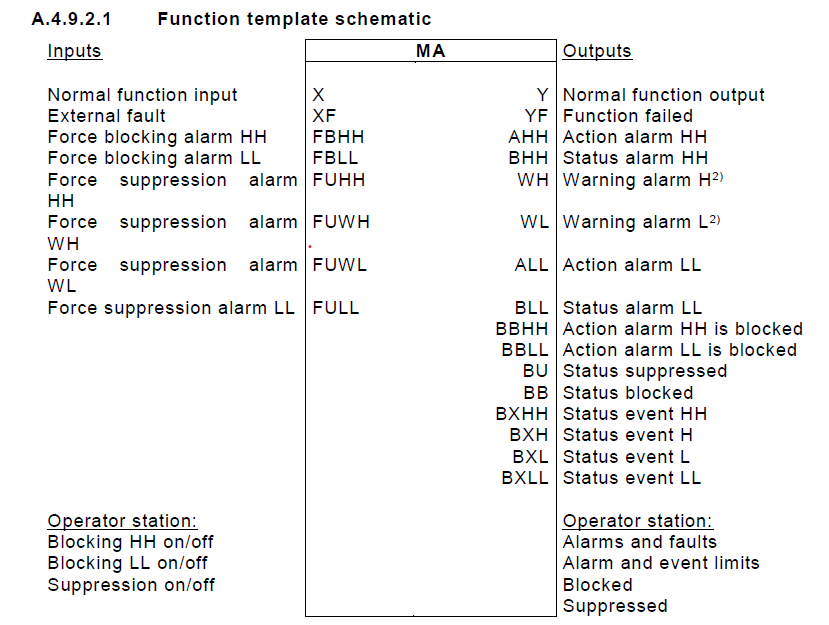
\includegraphics[width=1\textwidth]{Bilder/MABlokkIEC.png}
        \caption{IEC}\label{fig:Monitor Analogue blokk IEC}
    \end{subfigure}
    \hfill
    \begin{subfigure}[b]{0.45\textwidth}
        \centering
        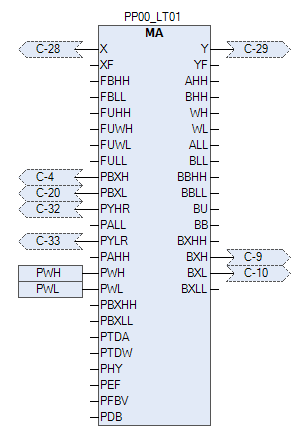
\includegraphics[width=0.7\textwidth]{Bilder/MABlokkIProgrammet.png}
        \caption{Bruk i programmet}\label{fig:Monitor Analogue blokk i programmet}
    \end{subfigure}
    \caption{Monitor Analogue}\label{fig:Monitor Analogue}
\end{figure}
\newpage

\subsection{Monitor Binary}

\gls{MB} funksjonsblokk blir brukt til automatisk overvåking, alarmhandtering, framvising og latching av binære prosess variablar.
Funksjonsblokka inkluderer alarm suppression og blocking funksjonalitet. Funksjonsblokka har moglegheit for invertering av 
inngangssignal og moglegheit for tidsforsinkelse av utgangssignal via parameter.

funksjonsblokka er brukt i programmet for å overvåke alle digitale nivåfølerar i prosessen.

\begin{figure}[htbp]
    \centering
    \begin{subfigure}[b]{0.45\textwidth}
        \centering
        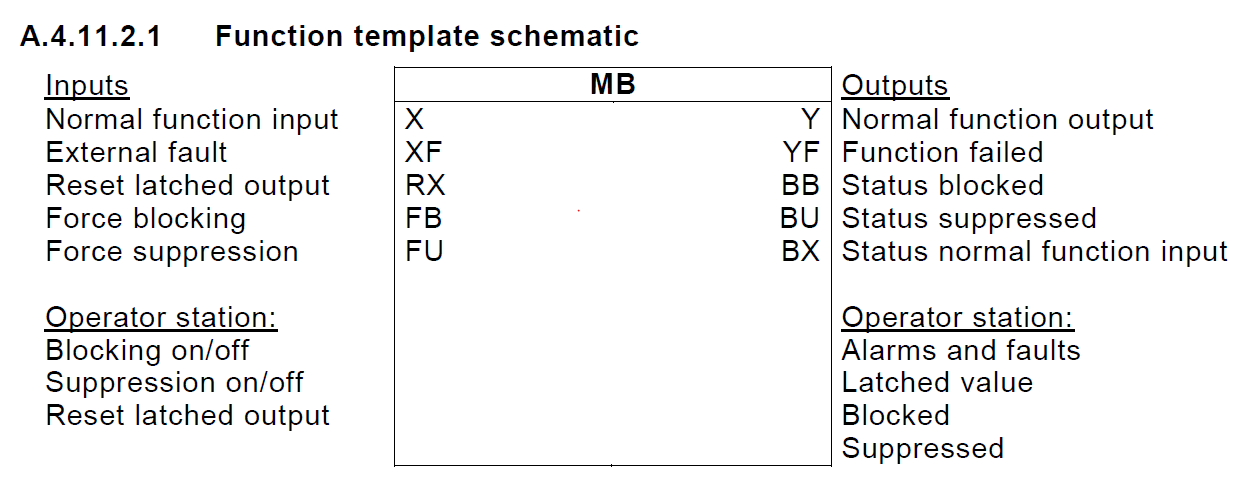
\includegraphics[width=1\textwidth]{Bilder/MBBlokkIEC.png}
        \caption{IEC}\label{fig:Monitor Binary blokk IEC}
    \end{subfigure}
    \hfill
    \begin{subfigure}[b]{0.45\textwidth}
        \centering
        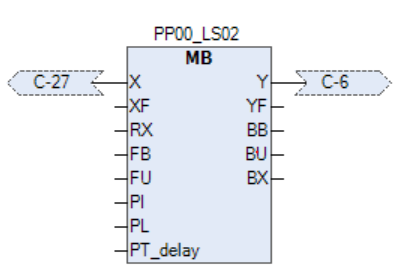
\includegraphics[width=0.7\textwidth]{Bilder/MBBlokkIProgrammet.png}
        \caption{Bruk i programmet}\label{fig:Monitor Binary blokk i programmet}
    \end{subfigure}
    \caption{Monitor Binary}\label{fig:Monitor Binary}
\end{figure}

\newpage

\subsection{Switch Binary Value}

\gls{SBV}-funksjonsblokka skal brukast til binær (på/av) kontroll av eit flyt element ved å endra straumen av medium (varme eller væske). 
Typisk kontrollerte element er ventilar, spjeld, osv.
Funksjonsblokka er brukt i programmet til og styre ventilar.

Funksjonsblokka skildrar kontrollen av ventilar med dei binære inngangane XH og XL.
Det er ein utgang Y, som formidlar eit opne/lukke (høg/låg) kommando til ventilaktivatoren,
eller dei pulserte utgangane YH og YL kan brukast. Funksjonsblokka har også utgonger XGH og XGL som bekreftar at ventil har fått høg eller låg tilbake melding frå ventilen.
Forklaringa på kontrollfunksjonane (rektangla) er som følgjer: "Kontrollfunksjon":Denne funksjonen utfører fleire oppgåver.
\begin{itemize}
    \item Den genererer feilstatus YF dersom ein ekstern eller intern feil blir rapportert
    \item Den set utgangen Y i samsvar med parameter når feil blir oppdaga;
    \item Den set utgangen Y basert på tilbakemelding i ytremodus når ingen eksterne inngangar blir brukte (XOH/XOL).
\end{itemize}

Der er det mogleg og bruke inngongar som kan handtere Lock safeguarding Force safeguarding, force disable transition, Force blocking, Force suppression. Videre er det også inngangar for lock Auto, manuell og outside.
Samt utgonger for som bekreftar status blocked, suppressed, auto/man og outside.

\begin{figure}[htbp]
    \centering
    \begin{subfigure}[b]{0.45\textwidth}
        \centering
        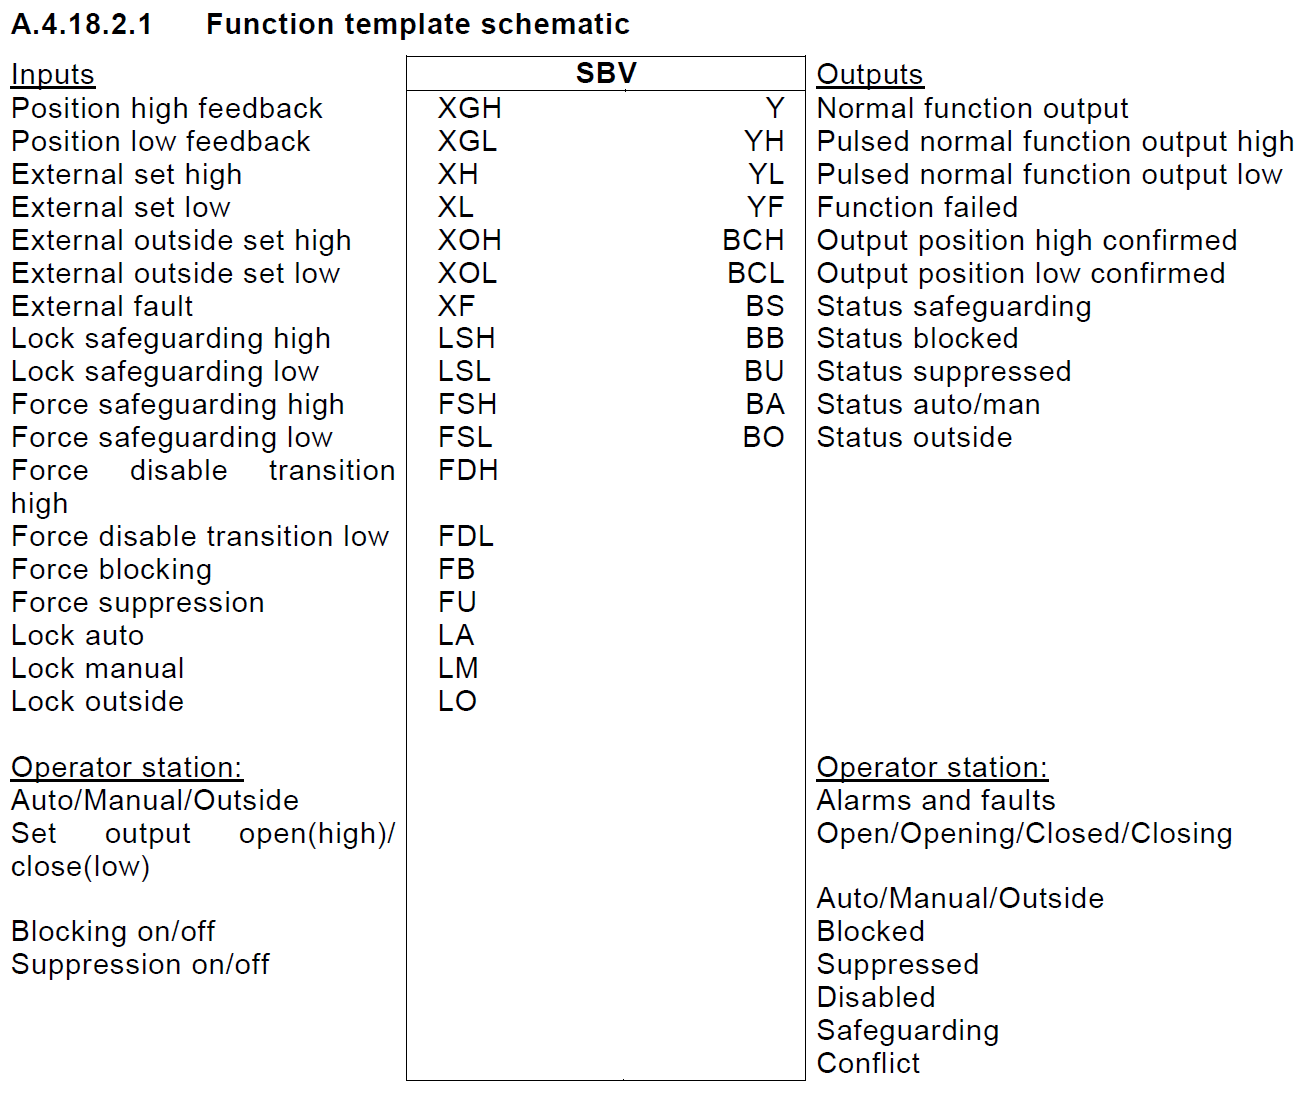
\includegraphics[width=1\textwidth]{Bilder/SBVBlokkIEC.png}
        \caption{IEC}\label{fig:Switch Binary Value blokk IEC}
    \end{subfigure}
    \hfill
    \begin{subfigure}[b]{0.45\textwidth}
        \centering
        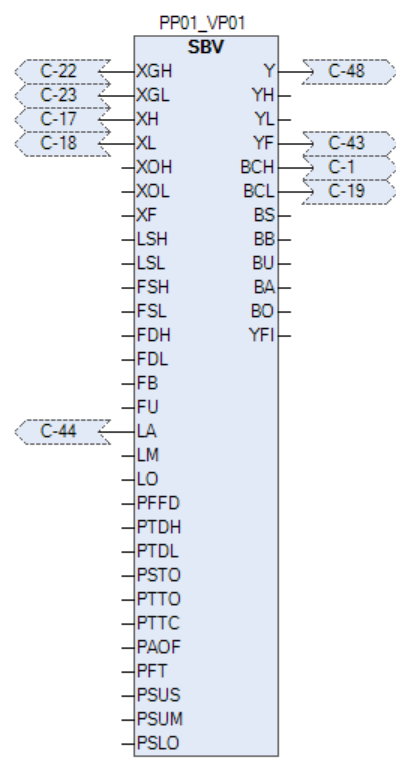
\includegraphics[width=0.5\textwidth]{Bilder/SBVBlokkIProgrammet.png}
        \caption{Bruk i programmet}\label{fig:Switch Binary Value blokk i programmet}
    \end{subfigure}
    \caption{Switch Binary Value}\label{fig:Switch Binary Value}
\end{figure}

\newpage

\subsection{Switch Binary Eletrical}

\gls{SBE} funksjonsblokka blir brukt for binærkontroll av straumningselement for elektrisitet, varme eller væske. Det
kontrollerte elementet er av typen motor, pumpe, varmeelement, vifte etc.

SBE blokka beskriver korleis ein kontrollarar ein enhet, for eksempel ein motor, pumpe, varmeelement, vifte etc.
Det er ein utgang Y, som gir ein opne/lukke (høg/lav) kommando til enheten. Blokka har fleire funksjonar, der den
tar output og samanliknar med tilbakemelding og gir korrekt BCL/BCH status. Den genererer også ein feil status på
YF om ein har ein ekstern feil inn.
Funksjonsblokka inkluderer alarm suppression, blocking, safeguarding og transition funksjonalitet.

\begin{figure}[htbp]
    \centering
    \begin{subfigure}[b]{0.45\textwidth}
        \centering
        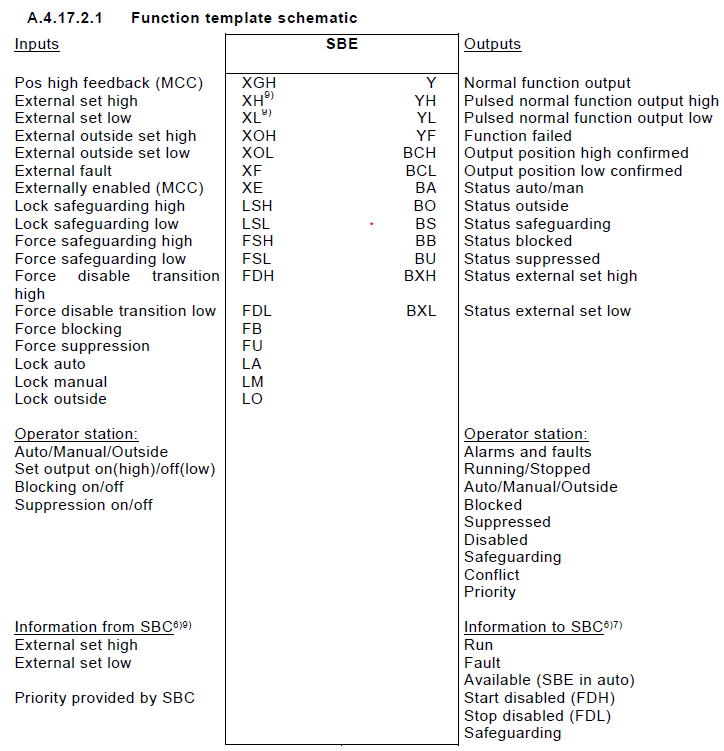
\includegraphics[width=1\textwidth]{Bilder/SBEBlokkIEC.png}
        \caption{IEC}\label{fig:Switch Binary Eletrical blokk IEC}
    \end{subfigure}
    \hfill
    \begin{subfigure}[b]{0.45\textwidth}
        \centering
        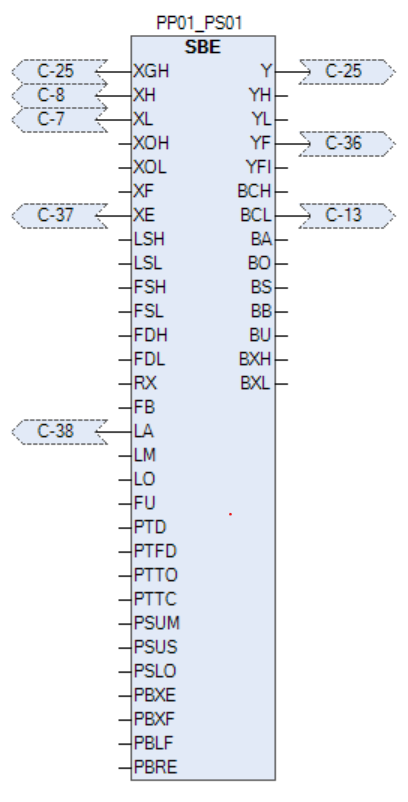
\includegraphics[width=0.5\textwidth]{Bilder/SBEBlokkIProgrammet.png}
        \caption{Bruk i programmet}\label{fig:Switch Binary Eletrical blokk i programmet}
    \end{subfigure}
    \caption{Switch Binary Eletrical}\label{fig:Switch Binary Eletrical}
\end{figure}

\newpage

%\begin{figure}[htbp]
%    \centering
%    \begin{subfigure}[b]{0.45\textwidth}
%        \centering
%        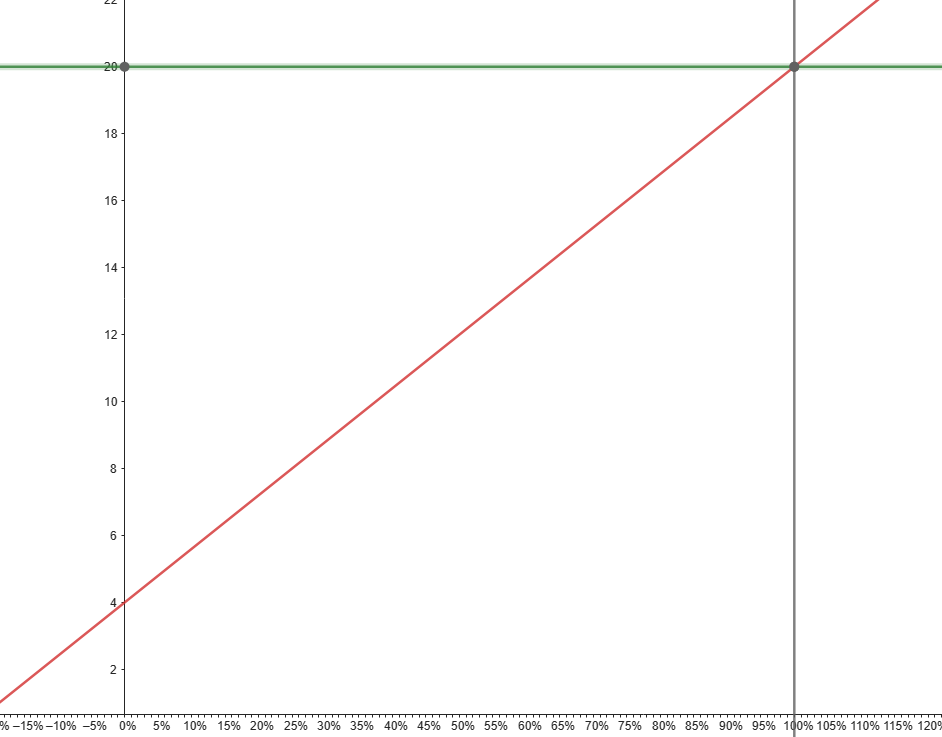
\includegraphics[width=1\textwidth]{Bilder/4_20mA_Scaling.png}
%        \caption{Skalering av mA mot prosent}\label{fig:Skalering av mA mot prosent}
%    \end{subfigure}
%    \hfill
%    \begin{subfigure}[b]{0.45\textwidth}
%        \centering
%        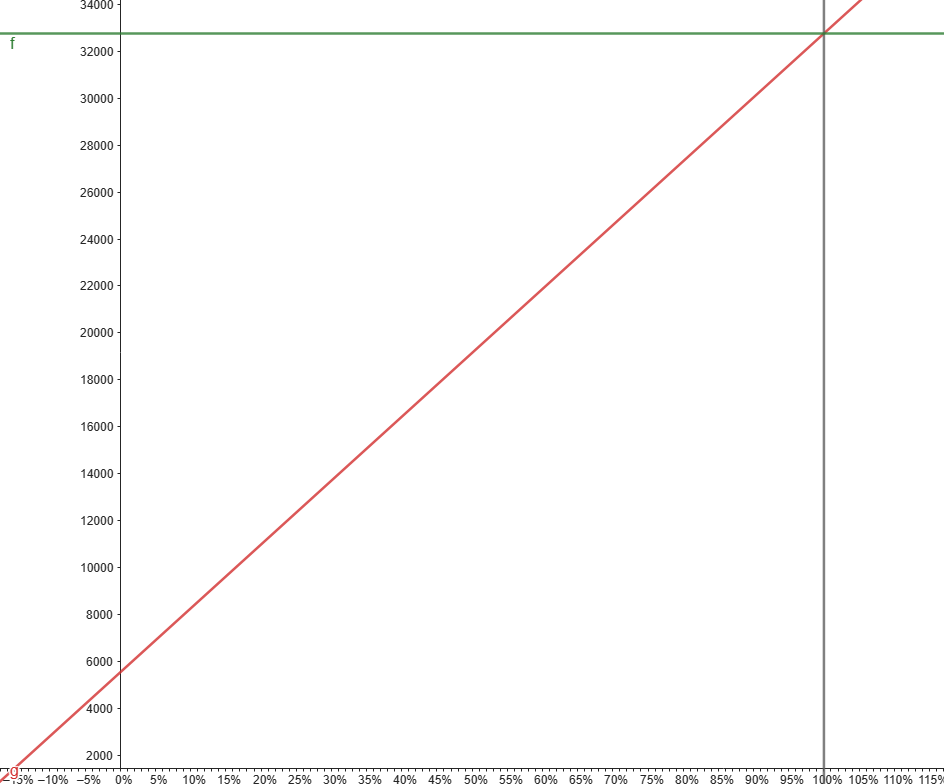
\includegraphics[width=0.95\textwidth]{Bilder/27327_prosent_Scaling.png}
%        \caption{Skalering av prosent til verdi}\label{fig:Skalering av prosent til verdi}
%    \end{subfigure}
%    \caption{Dei forskjellige skaleringane av inngangssignal}\label{fig:Skalering av prosent til verdi}
%\end{figure}

